\chapter{Data Description and Preprocessing}
\label{ch:data}

\section{Data description}
In this project, we mainly investigate the stock market in America, since the relevant data are relatively complete and free to use. In particular, the dataset used in this project is \hyperlink{https://www.kaggle.com/borismarjanovic/price-volume-data-for-all-us-stocks-etfs}{Huge Stock Market Dataset} (accessed in May 8th 2021). This dataset contains full price and volume records of 7195 different stocks from 1977 to 2017 for all stocks trading on the NYSE, NASDAQ, and NYSE MKT. Each record has 6 attributes: \textbf{Date:} the date of that record; \textbf{Open:} the opening price of the stock at that day; \textbf{High:} the highest stock price of that day; \textbf{Low:} the lowest stock price of that day; \textbf{Close:} the closing price of the stock of that day; \textbf{Volume:} the total number of shares traded of that day. In the original dataset, there is an additional attribute ``OpenInt'', however, since there is no actual record of it, this attribute is discarded. In addition, the ``Volume'' attribute is not directly associated with stock price, therefore, it is also discarded in this project. The final representation of a single stock can be regarded as a 2-dimensional tensor with its first dimension corresponding to the time axis and the second dimension representing features. Note that due to some factors such as the regular suspension of stock market, there could be no records in some periods. Consider that mining the whole dataset could be time-consuming, merely 5 years records from Jan 1st 2011 to Dec 31th 2015 of 100 companies are used in this project. Figure \ref{fig:curve1} and \ref{fig:candlestic1} show the price curve and candlestick chart of `IBA' stock in 2011 respectively, x-axis represents the trading days while y-axis represents the prices.
\begin{figure}[!htbp]
    \centering 
    \subfigure[Curve chart] { \label{fig:curve1} 
    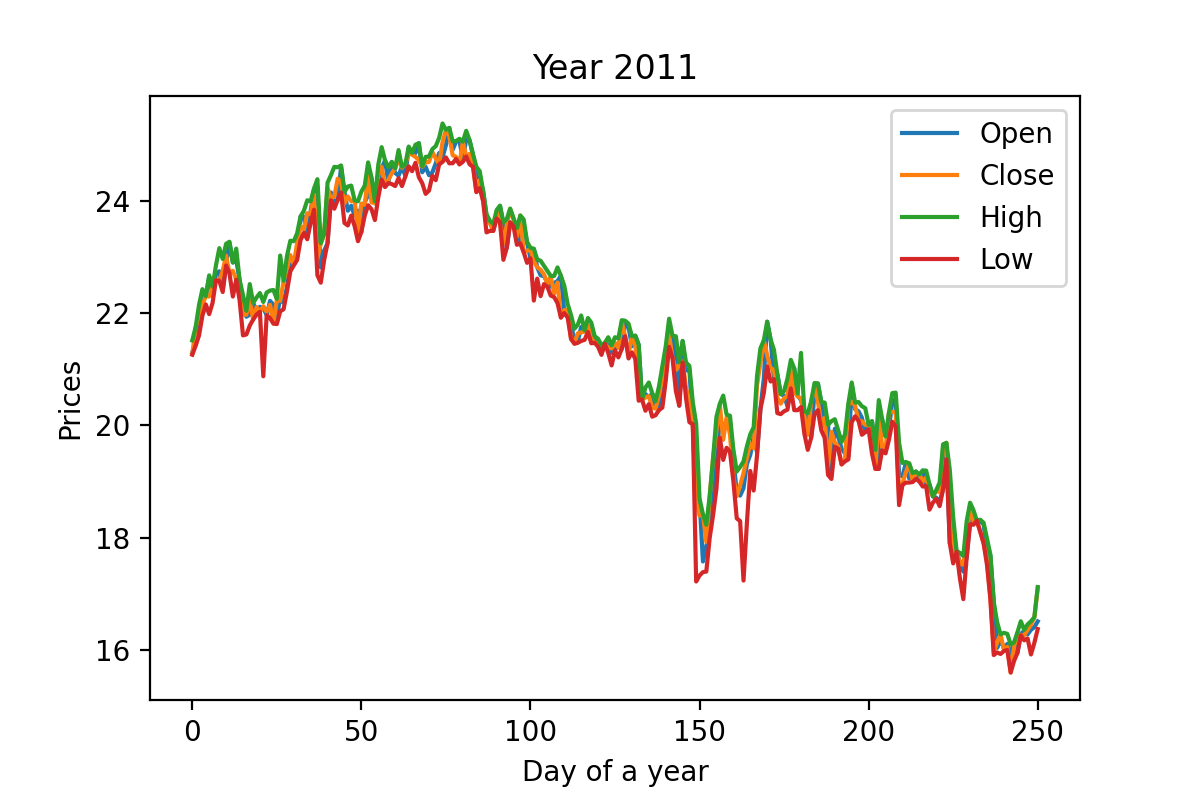
\includegraphics[width=0.4\columnwidth]{sample1.png} 
    } 
    \subfigure[Candlestick chart] { \label{fig:candlestic1} 
    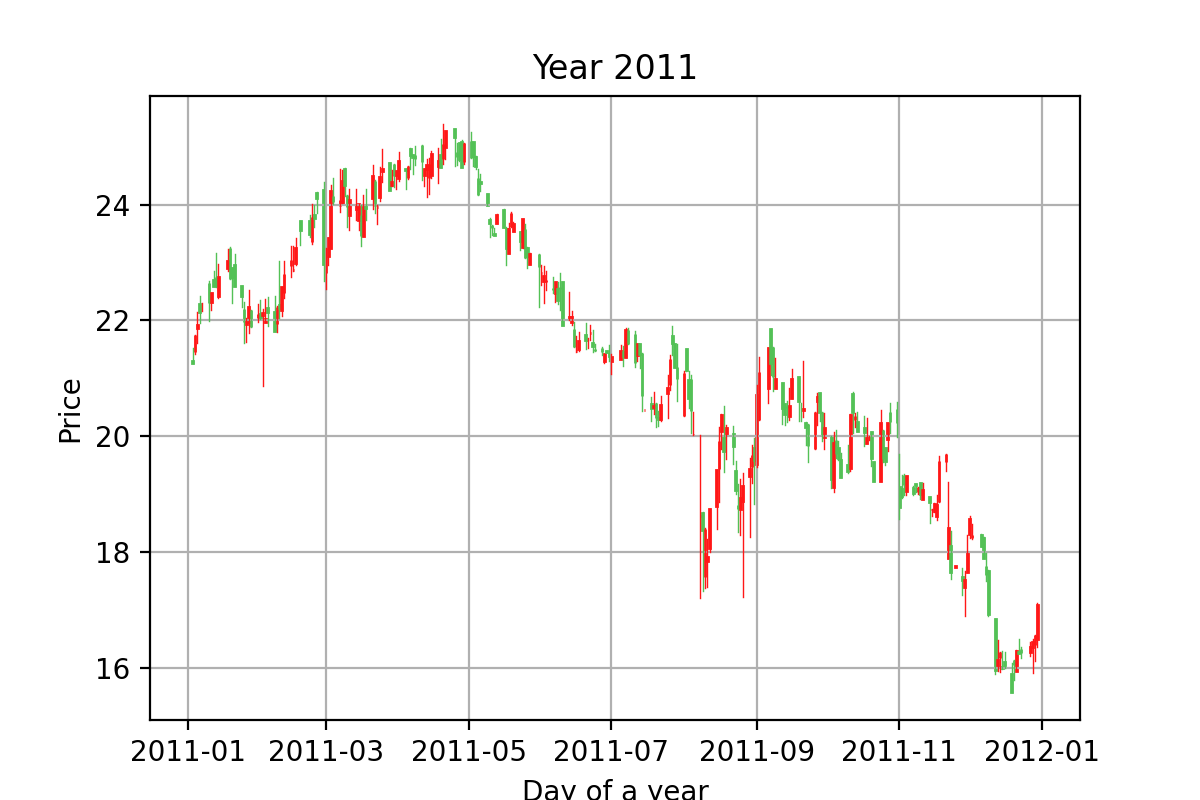
\includegraphics[width=0.4\columnwidth]{kline1.png} 
    } 
    \caption{ Sample data } 
    \label{fig:sample1} 
\end{figure} 

\section{Time-series preprocessing}
As mentioned in Section~\ref{sec:invariance}, we want the data being transformed into a new form with 5 invariances before feeding them to clustering algorithms. According to \cite{paparrizos2015k}, some of those invariances can be achieved by preprocessing the data. This section describes some common approaches to preprocess time series data and how we process the data to eliminate the certain distortions.

\subsection{Time-series denoising}
\label{sec:denosing}
Sequence denoising is closely related to the \textbf{complexity invariance} mentioned in Section~\ref{sec:invariance}. Due to numerous factors, stock price sequences contains many noises (i.e. short-term volatility). Such noises could make some distance measurement inaccurate, for example, in terms of dynamic time warping (DTW), the unsmoothed curve with many fluctuations could make the alignment process broken. Therefore, noisy sequences may have an obvious impact on the performance of clustering algorithms \cite{zhang2011novel}. For time series clustering problem, the continuous trend characteristics of data are hoped to be stable, and this can be achieved by filtering short-term noises. Since the time series data are non-linear and have high Signal to Noise Ratio, using traditional filters such as Gaussian filter and median filter could change the general shape of the sequences. In practical, the denoising of stock sequences is most done by Wavelet transform. Similar to fourier transform, Wavelet transform gives the frequency representation of a signal. The main difference is that the standard Fourier transform is merely localized in frequency while wavelets are localized in both time and frequency \cite{shensa1992discrete}, which means that with this transform, the low frequency band could have a lower time resolution and higher frequency resolution, while the higher frequency band could have a higher time resolution and lower frequency resolution \cite{wu2021hybrid}. The properties of Wavelet transform makes it appropriate for time series data decomposition.\\
\\Generally, the wavelet-based denoising process is done by \textbf{Discrete Wavelet Transforms (DWT)}. DWT  decomposes the signal into mutually orthogonal set of wavelets, each set describes the time evolution of the signal in the corresponding frequency band \cite{altunkaynak2016comparison}. Once the coefficients of each set is computed, they can be used to reconstruct the signal. Theoretically, noises are more sparse among all frequencies, the coefficients of important information are higher than that of noises, which makes the denoising possible. \\
\\Figure~\ref{fig:dwt1} shows the general pipeline of DWT-based denoising process. The main parameters of using such approach are the wavelet function and decomposition layers, in this project, we choose db4 as the wavelet function with decomposition layers set to 3. To verify the effectiveness of the denoising process, we compare the original sequences with the denoised version in terms of the similarity/distance measurement. Figure~\ref{fig:denoising1} visually proves that the denoising process improves the accuracy of sequences matching. In this set of figures, the records of two stocks with abbreviation ``WWW'' and ``HCCI'' in 2011 are used as an example. In general, these two stocks share a similar trend and are expected to have a small distance between them. As can be seen in Figure~\ref{fig:undenoised1}, the original sequences have many fluctuations, which makes the DTW alignment of two sequences inaccurate and disordered (see Figure~\ref{fig:denoised1}). After applying the denoising algorithm to them, these two sequences are smoothed while the general shapes are preserved, the number of points in each denoised sequence is also the same with the undenoised one. Moreover, it's obviously that the alignment result is improved. As mentioned before, the serration could make DTW alignment inaccurate, and the results in Figure~\ref{fig:undenoised2} and Figure~\ref{fig:denoised2} show that smoothing the curve can alleviate the problem. Numerically, the distance between the denoised sequences is 3.85, while that between the original sequences is 5.50, roughly 43\% larger. Similar improvement can be found in use of other distance metrics. Table~\ref{tab:denoising1} shows the results of denoising process conducted on 20 similar sequences. 4 different distance metrics are used to computed the distance between each pair, where the ``Cosine'' and ``Correlation'' are $1-\frac{X \cdot Y}{\Vert X \Vert \Vert Y \Vert}$ and $1-\frac{(X-\bar{X}) \cdot (Y-\bar{Y}) }{\Vert X-\bar{X} \Vert_2 \Vert Y-\bar{Y} \Vert_2}$. The values in the table are the arithmetical mean of 190 pairs. Note that the sequences used in this experiment are already normalised and compressed. As can be seen, all the four metrics are shortened, which proves that the denoising process can contribute to complexity invariance. \textbf{Same with \cite{wu2021hybrid}, we choose db8 with threshold parameter of 0.04 as the wavelet function.}
\begin{figure}[!htbp]
    \centering
    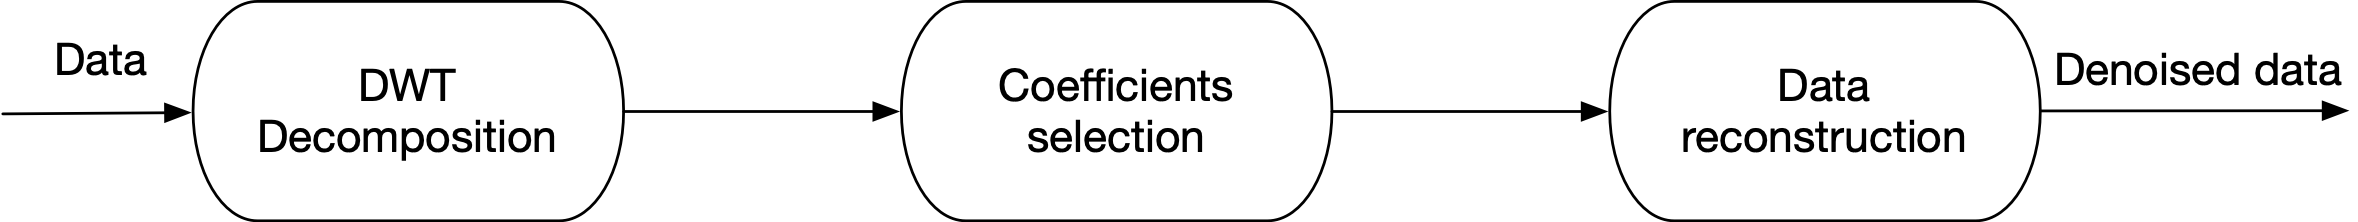
\includegraphics[width=5in]{DWT.png}
    \caption{DWT-based denoising process}
    \label{fig:dwt1}
\end{figure} 

\begin{figure}[!htbp]
    \centering 
    \subfigure[Original sequences] { \label{fig:undenoised1} 
    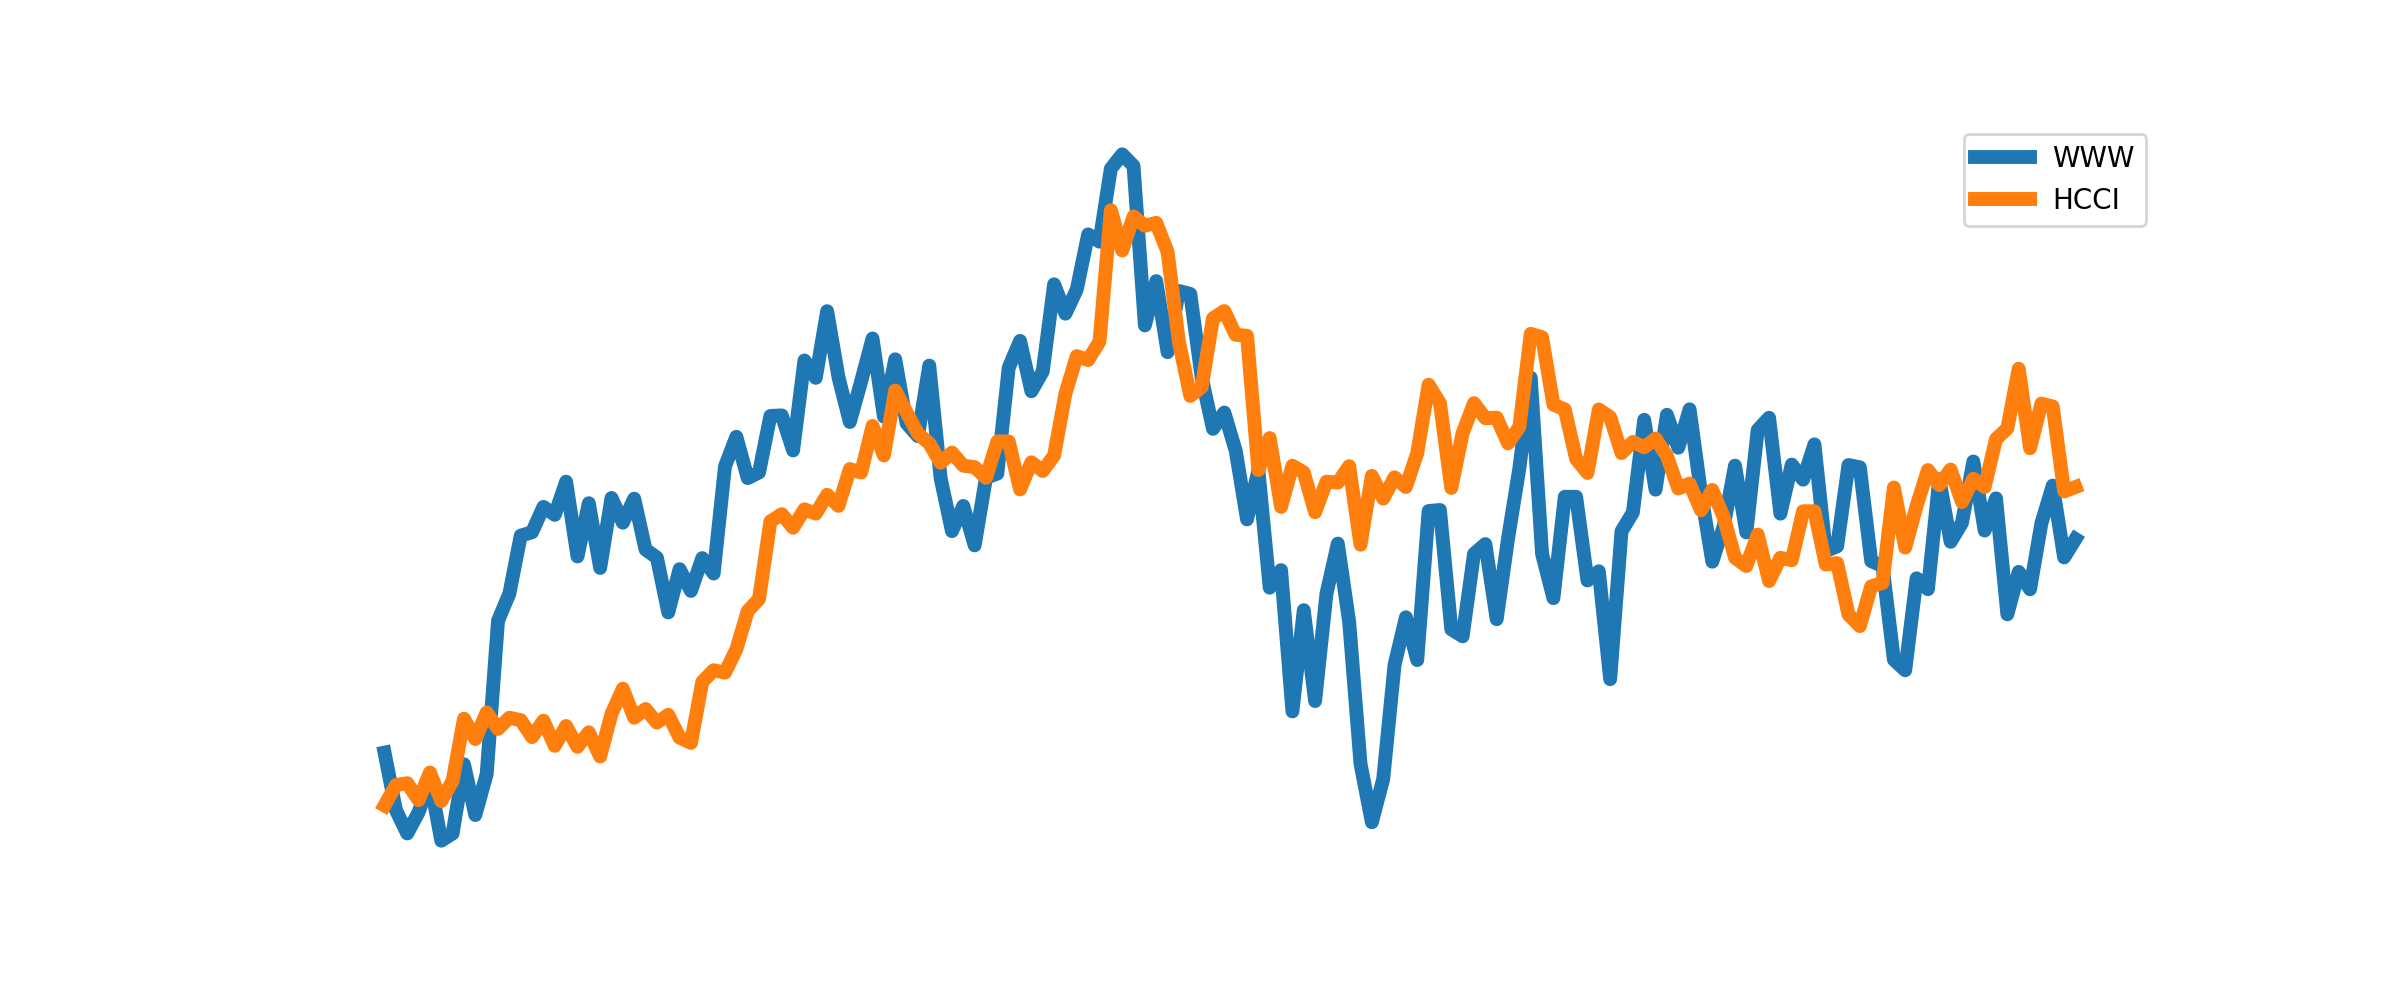
\includegraphics[width=0.45\columnwidth]{undenoised.png}} 
    \quad
    \subfigure[Denoised sequences] { \label{fig:denoised1} 
    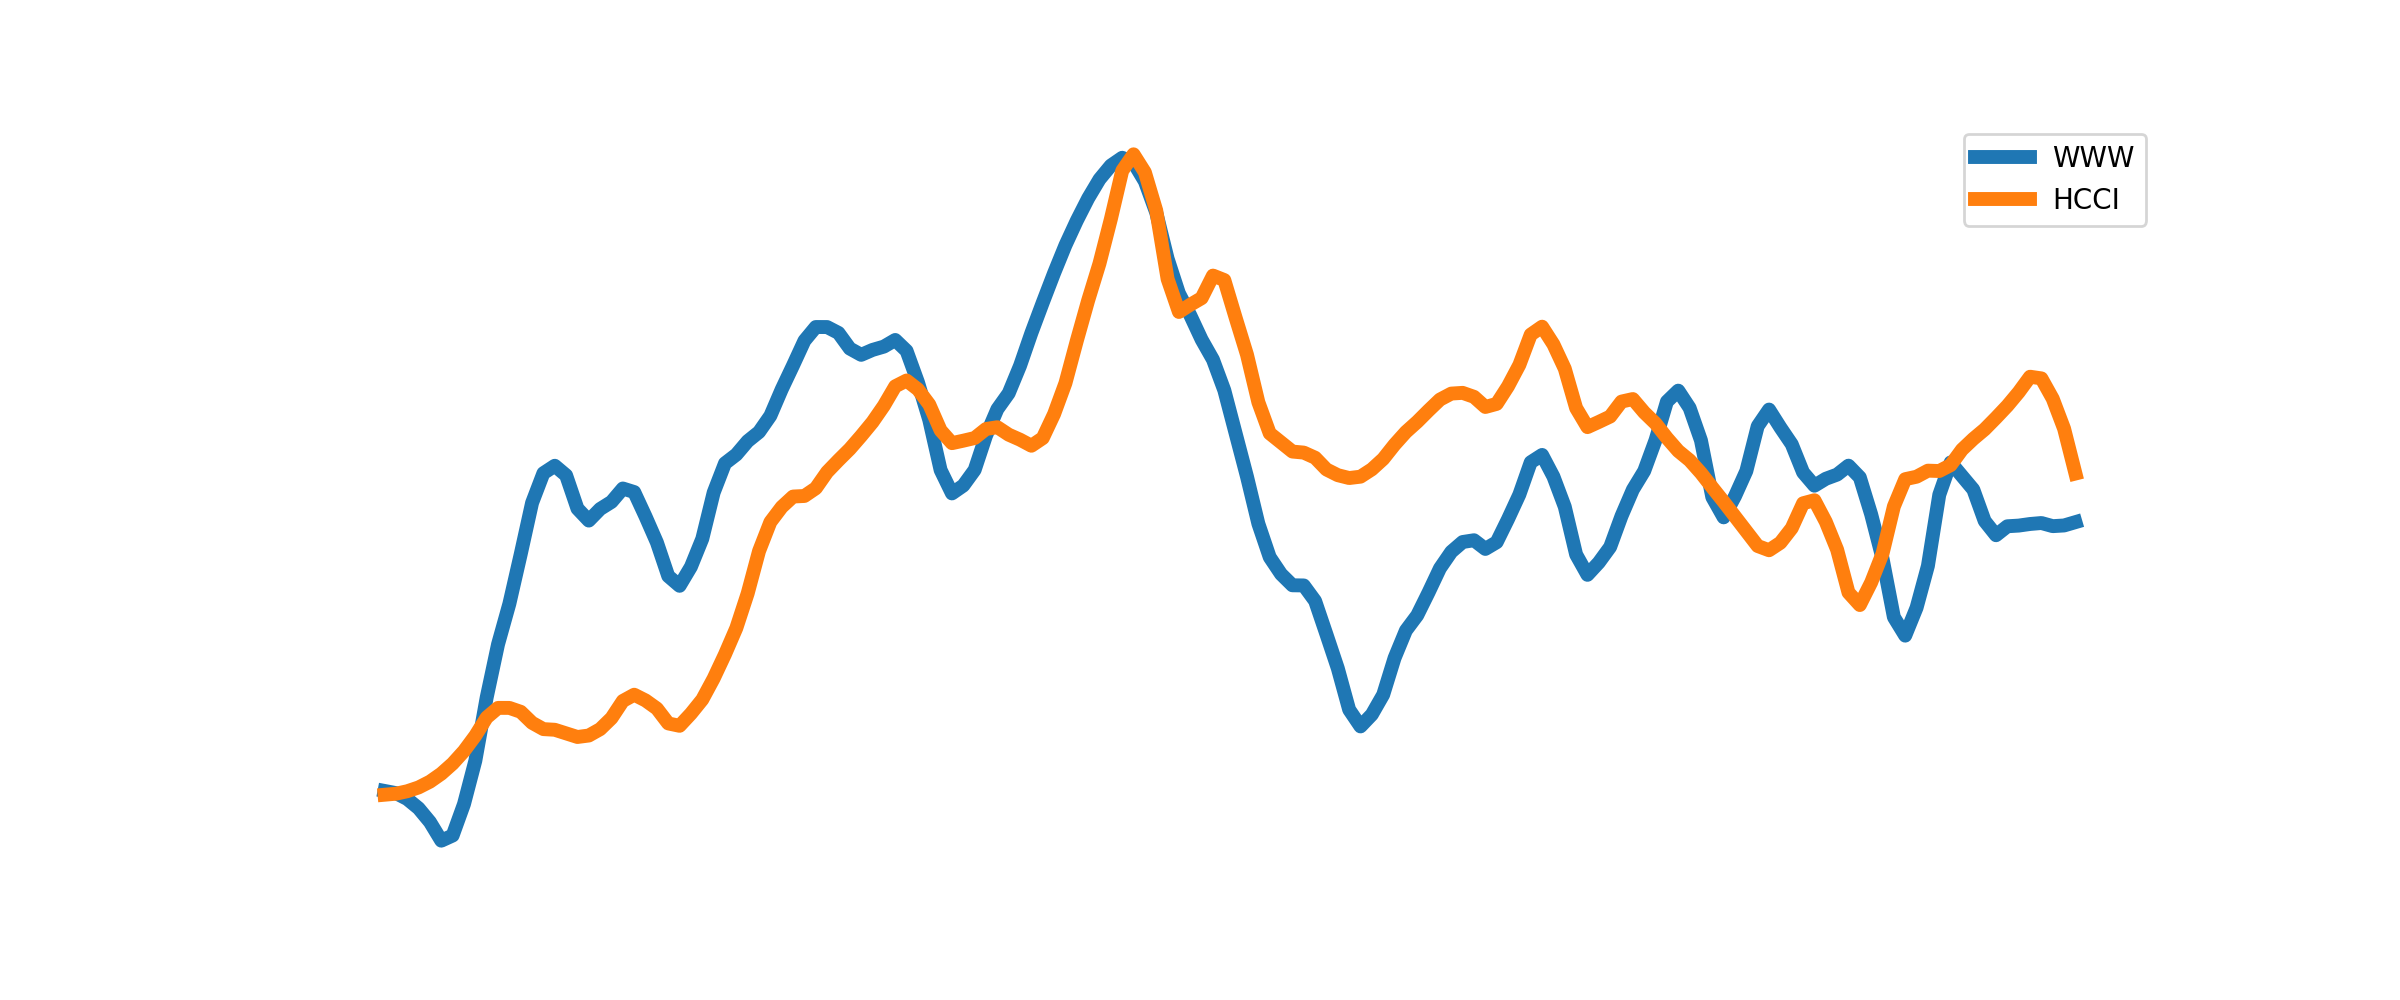
\includegraphics[width=0.45\columnwidth]{denoised.png} 
    } 
    \quad
    \subfigure[DTW Alignment of original sequences] { \label{fig:undenoised2} 
    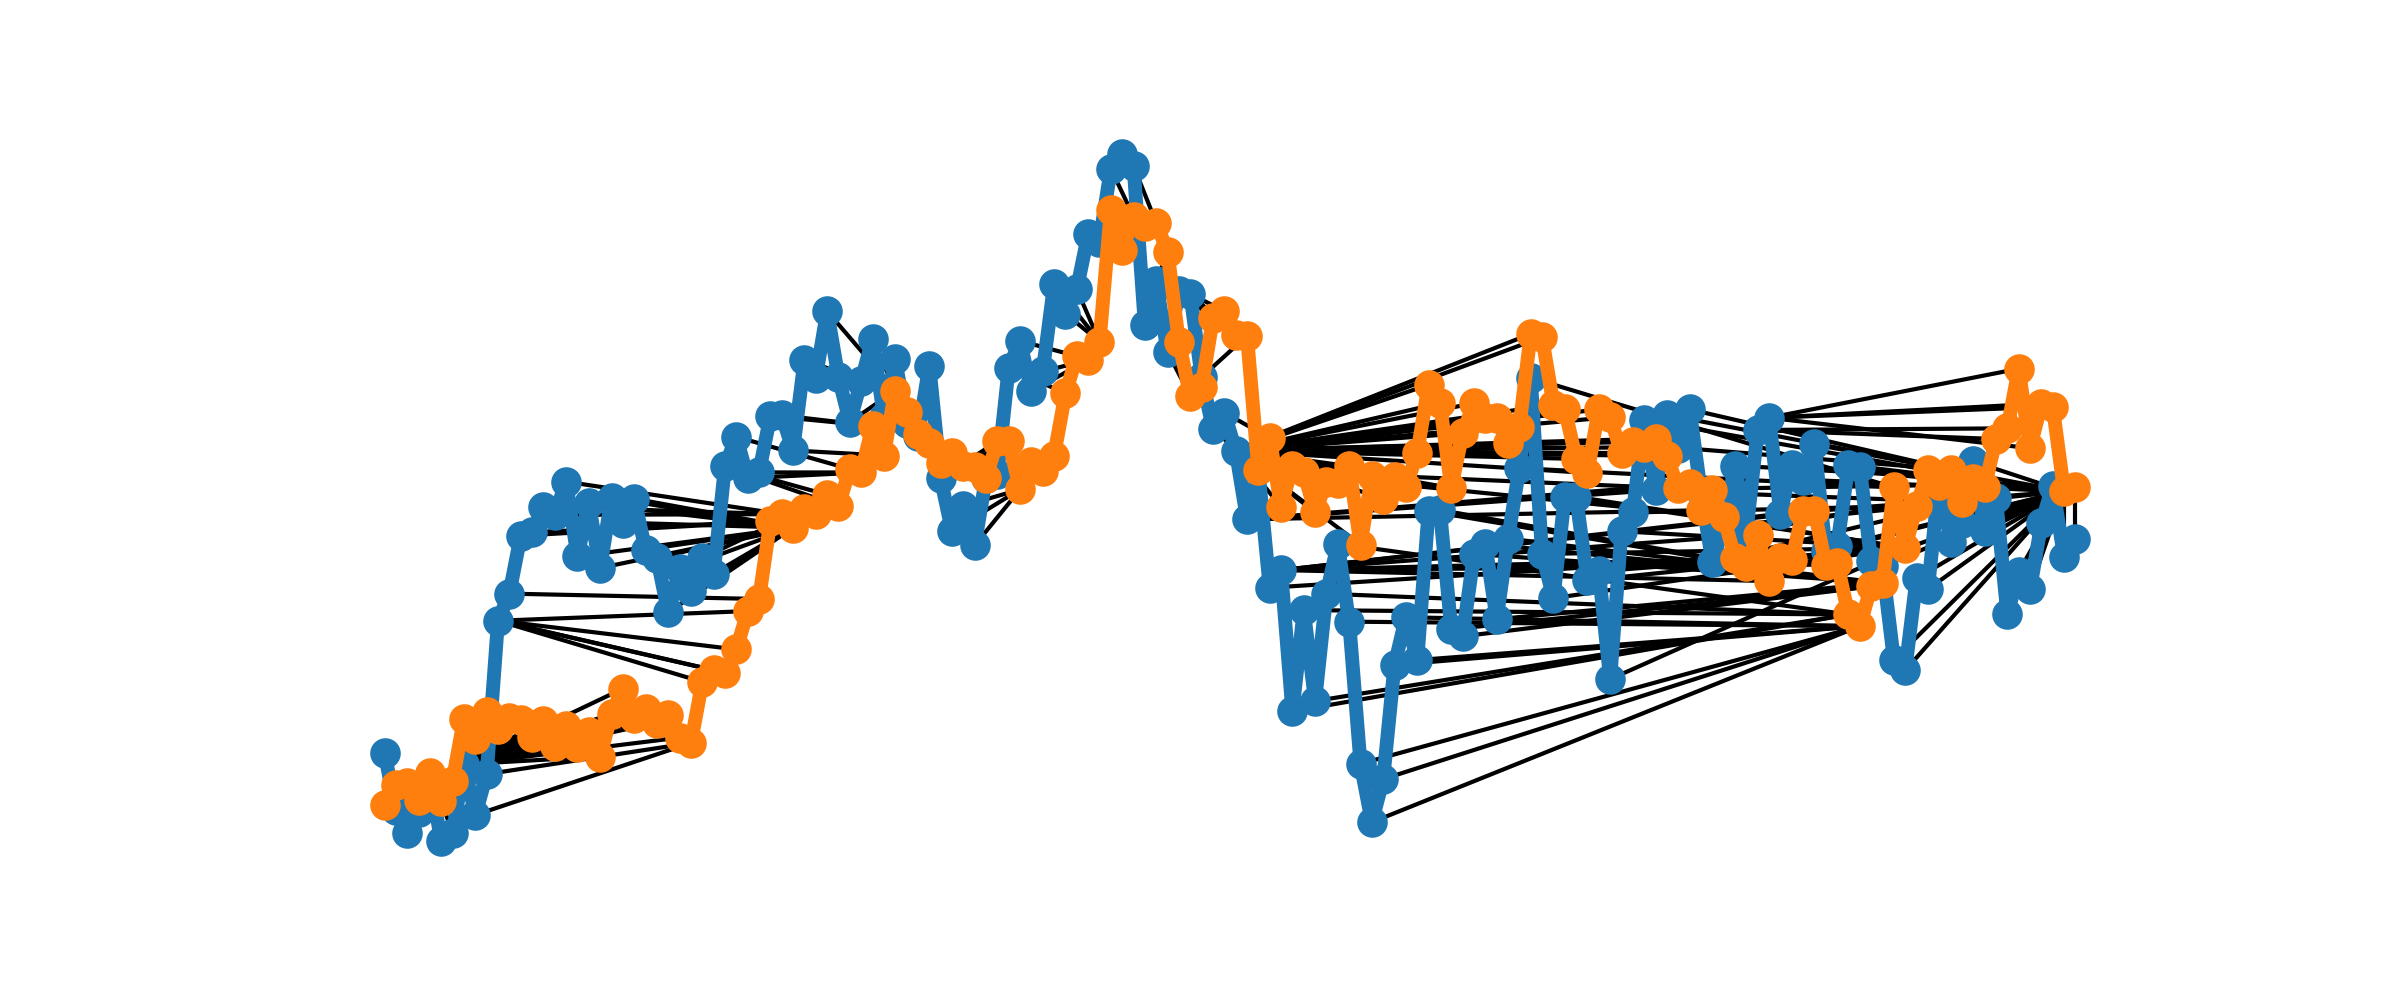
\includegraphics[width=0.45\columnwidth]{undenoised_dtw.png}}
    \quad
    \subfigure[DTW Alignment of denoised sequences] { \label{fig:denoised2} 
    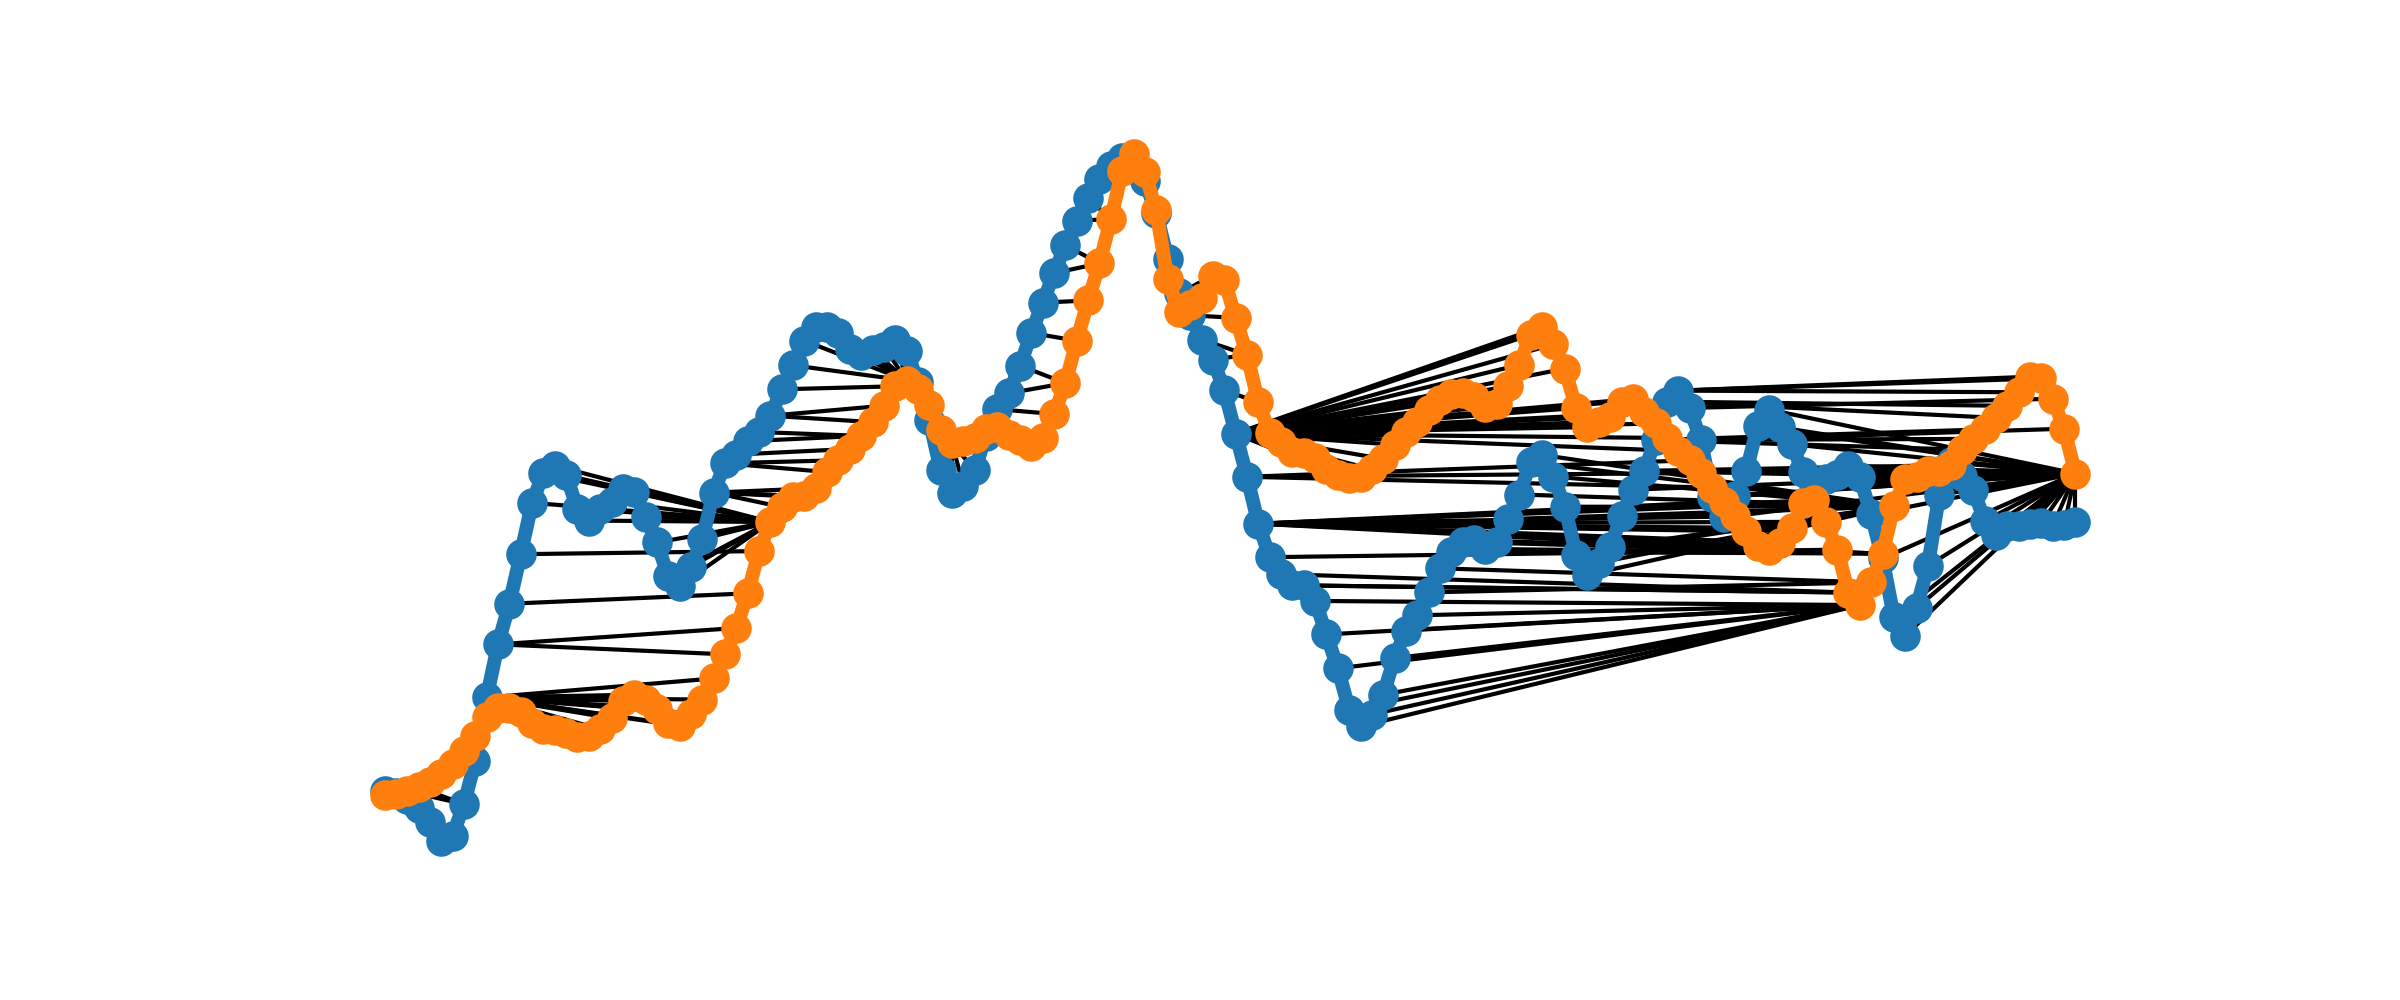
\includegraphics[width=0.45\columnwidth]{denoised_dtw.png}}

    \caption{ Sequences denoising results } 
    \label{fig:denoising1} 
\end{figure} 

\begin{table}[!htbp]
    \centering
    \hspace{0.5cm}
    \begin{tabular}{|c|c|c|c|c|}
        \hline
         & DWT & Cosine & Euclidean & Correlation \\ \hline
        Original & 3.442 & 0.168 & 6.743 & 0.168 \\ \hline
        Denoised & 3.382 & 0.161 & 6.541 & 0.161 \\ \hline
    \end{tabular}
    \caption{Sequences denoising results}
    \label{tab:denoising1}
\end{table}


\subsection{Time-serie normalization}
\label{sec:normalization}
Sequence normalization is the most simple and effective way to ensure \textbf{scaling and offset invariance} \cite{batista2014cid}. Each stock could have a unique movement range of its price, and such range could vary during different time periods. To eliminate the influence of the variance of vertical scaling and offset, data normalization is required. In this project, we mainly experiment with two most common normalization approaches used in machine learning -- Min-Max normalization and Z-Score normalization. Min-Max normalization could scale the data into range [0,1] while preserving the general shape. The equation of this approach is listed in \ref{equ:minmax}. It guarantees that all features will have the exact same scale. The main drawback of this normalization is that it can not handle outliers well. Assuming that there are 99 data points locating in value range [0,40] and one point has value 100, then the 99 points will be transformed into value range [0,0.4], leading to a squashed distribution. To the contrary, Z-Score normalization can avoid outlier issue. Its formula is listed in \ref{equ:zerosmean}, where $\mu$ stands for the mean value of the feature and $\sigma$ stands for the standard deviation of the feature. different from Min-Max normalization, this normalization could result in negative values: values greater than $\mu$ will be postive numbers while values less than $\mu$ will be negative numbers. The main drawback of Z-Score normalization is that it can not guarantee the transformed data have the exact same scale. Different from other data, for time series data, the normalization is usually applied to each individual.\\
\\Figure~\ref{fig:normalization1} shows the results of using these two approaches. As can be seen, both of them preserve the shape of original sequence (see Figure~\ref{fig:sample1}) in different scale. Mathematically, both of them can guarantee scaling and offset invariance. But in experiment we find that using the exact same scaling could be inappropriate. Figure~\ref{fig:scaling1} shows an example of that. Sequence 1 (colored with blue) ranges between 3.0 and 5.5 while sequence 2 (colored with orange) ranges from 20.0 to 30.0. They shares a roughly similar shape when examine them individually (as shown in the top middel and top right). However, as you may find in Figure~\ref{fig:subscaling1}, if we examine them together, the difference is significant. This indicates that scaling matters in time series tasks. After Min-max normalization, they locate in a same range (see bottom left), and hence they are categorized into a same cluster. From our perspective, such result is incorrect. \textbf{To take the scaling into consideration, we choose the Z-Score normalization as the normalization strategy.}

\begin{equation}
    x_i^{\prime} = \frac{x_i - \min_{i\leq j \leq n} \{x_j\}}{\max_{i\leq j \leq n} \{x_j\} - \min_{i\leq j \leq n} \{x_j\} }
    \label{equ:minmax}
\end{equation}

\begin{equation}
    x_i^{\prime} = \frac{x_i - \mu}{\sigma}
    \label{equ:zerosmean}
\end{equation}

\begin{figure}[!htbp]
    \centering 
    \subfigure[Min-Max normalization] { \label{fig:minmax1} 
    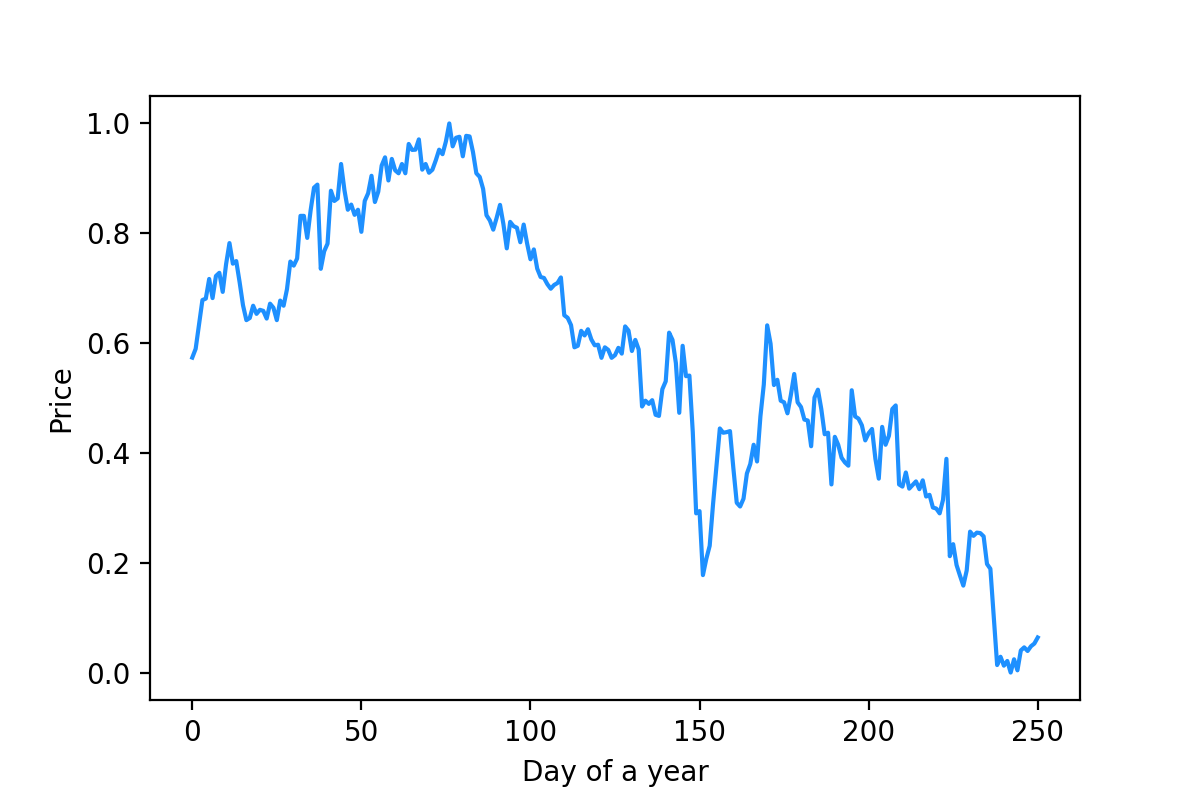
\includegraphics[width=0.3\columnwidth]{minmax.png} 
    } 
    \subfigure[Z-Score normalization] { \label{fig:zeromean1} 
    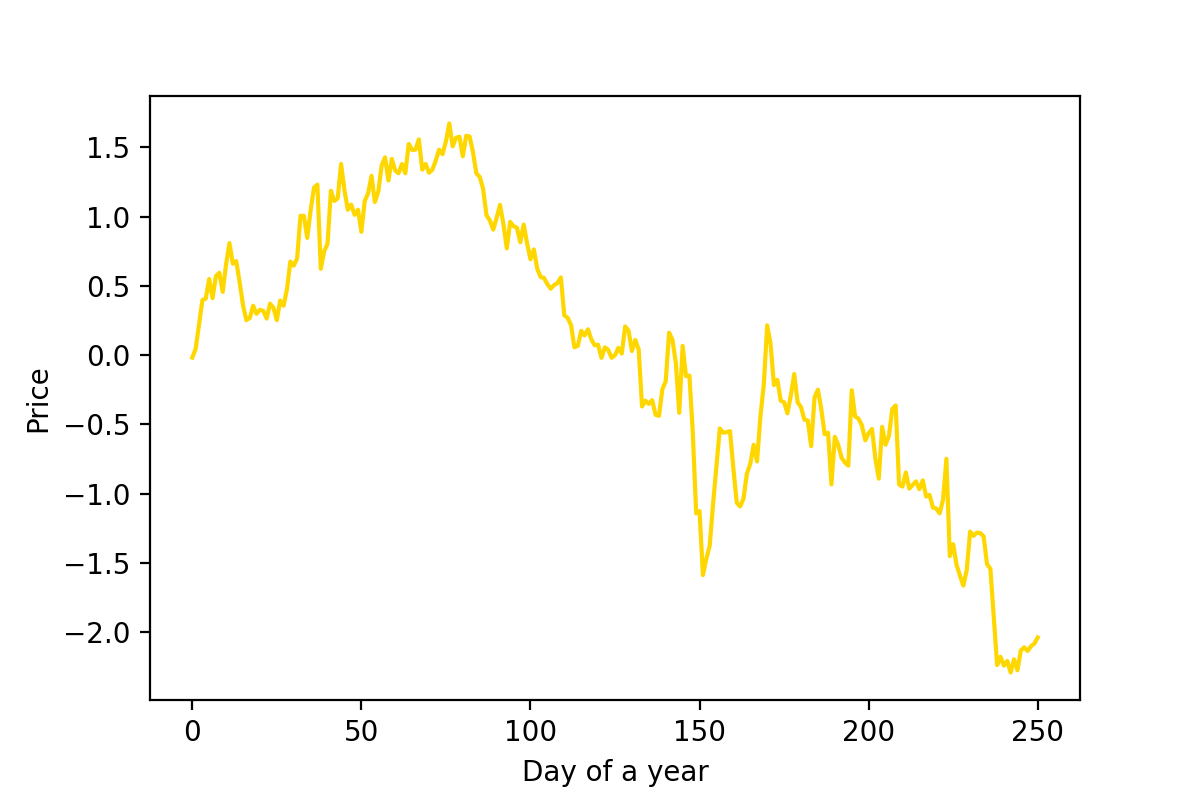
\includegraphics[width=0.3\columnwidth]{zmeans.png} 
    }
    \subfigure[Comparison] { \label{fig:minzero1} 
    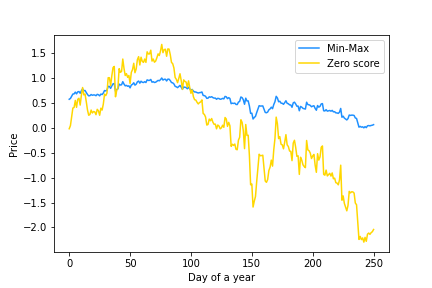
\includegraphics[width=0.3\columnwidth]{minzero.png} 
    }  
    \caption{ Results of normalization } 
    \label{fig:normalization1} 
\end{figure} 
\begin{figure}[!htbp]
    \centering 
    \subfigure[Original sequences] { \label{fig:subscaling1} 
    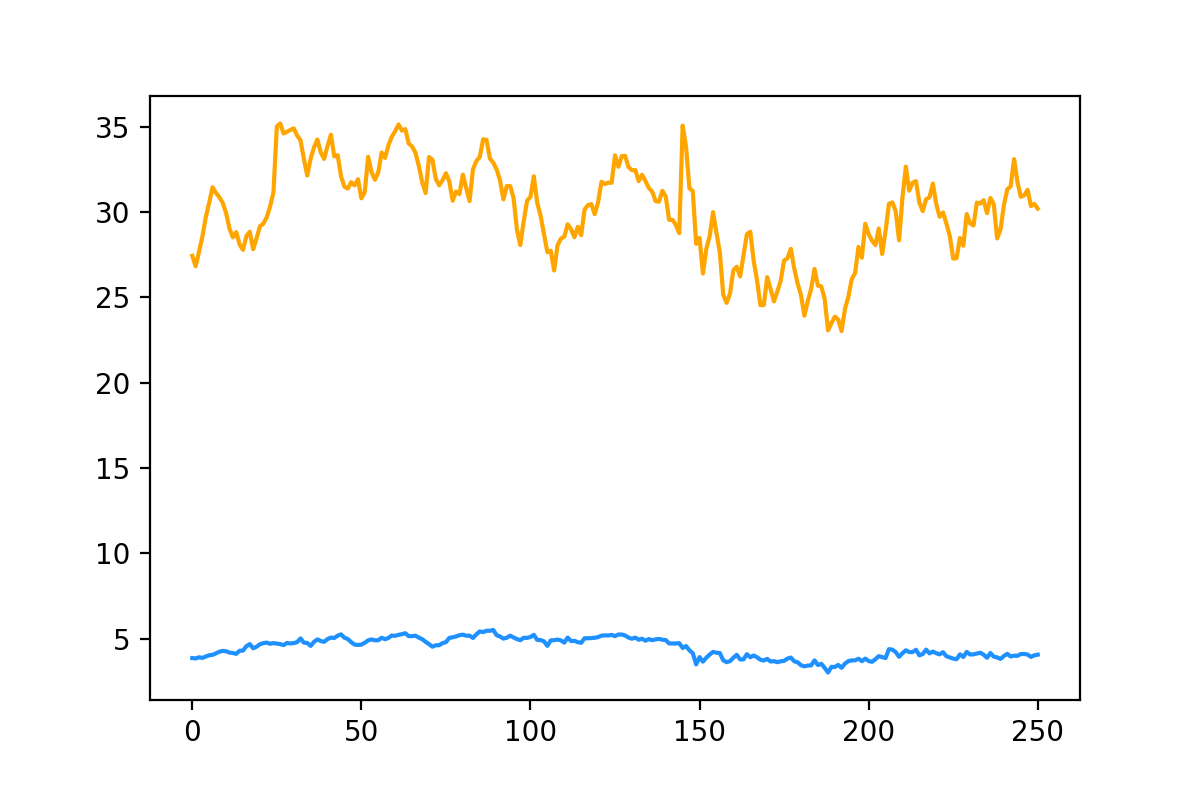
\includegraphics[width=0.3\columnwidth]{scaling1.png} 
    } 
    \subfigure[Sequence 1] { \label{fig:subscaling2} 
    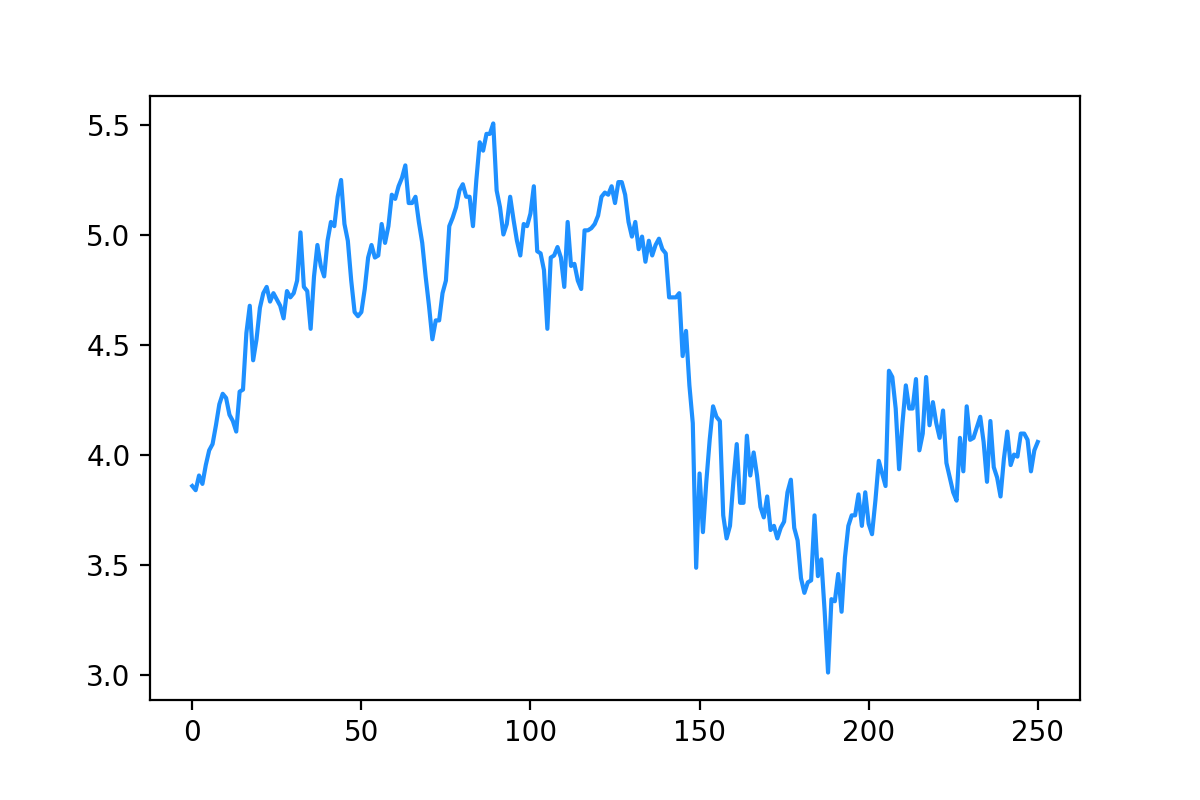
\includegraphics[width=0.3\columnwidth]{scaling2.png} 
    }
    \subfigure[Sequence 2] { \label{fig:subscaling3} 
    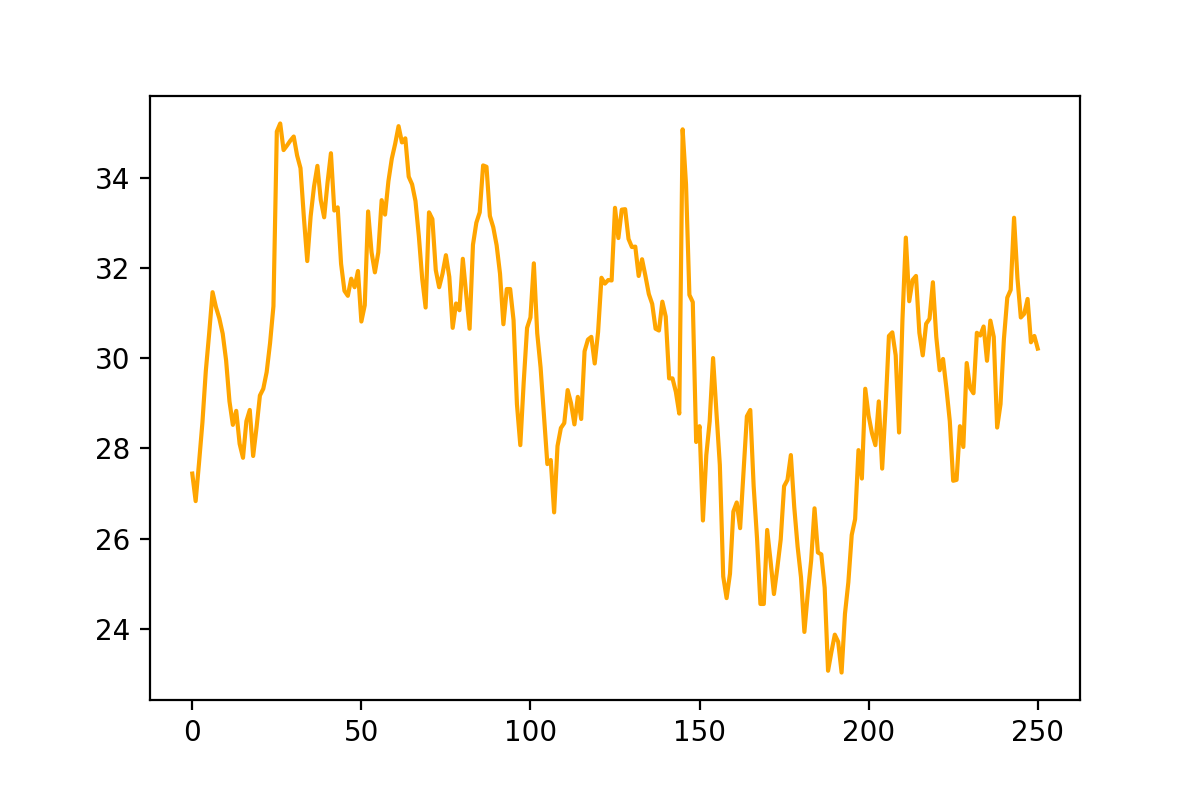
\includegraphics[width=0.3\columnwidth]{scaling3.png} 
    } 
    \subfigure[Min-Max normalization] { \label{fig:subscaling4} 
    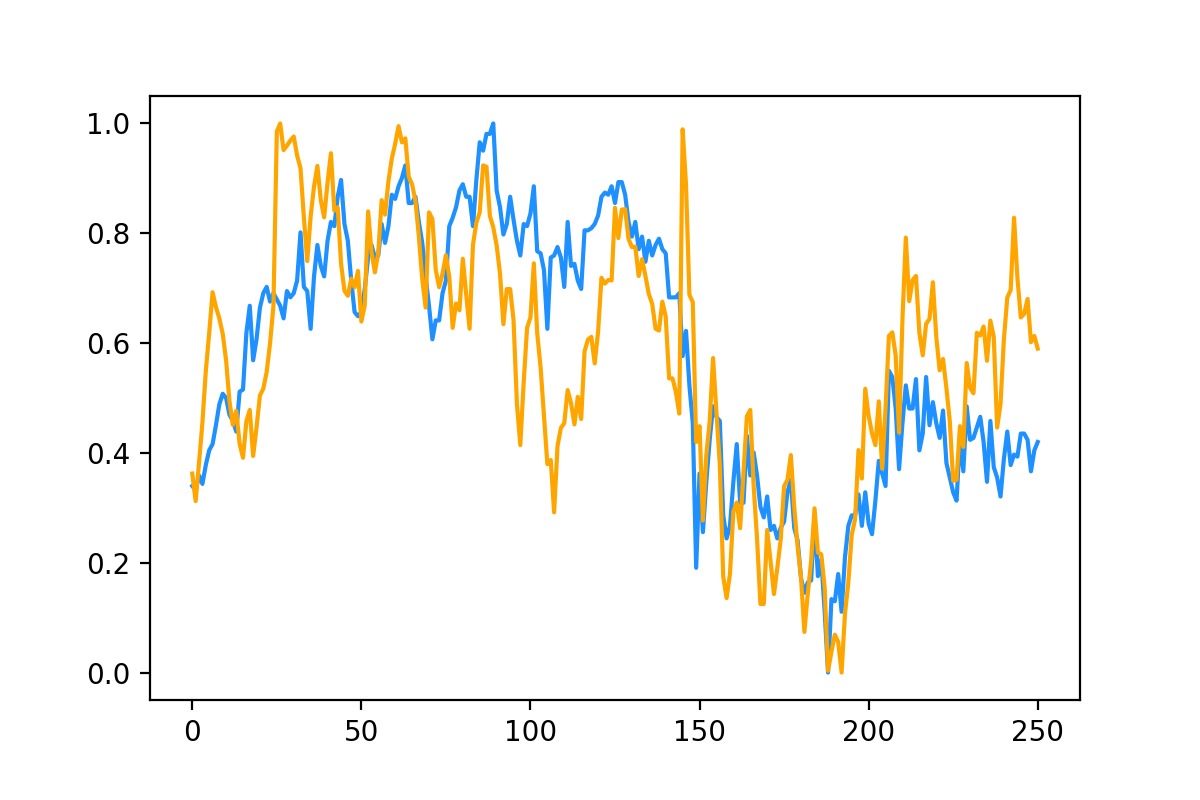
\includegraphics[width=0.3\columnwidth]{minmax2.png} 
    }
    \subfigure[Z-Score normalization] { \label{fig:subscaling5} 
    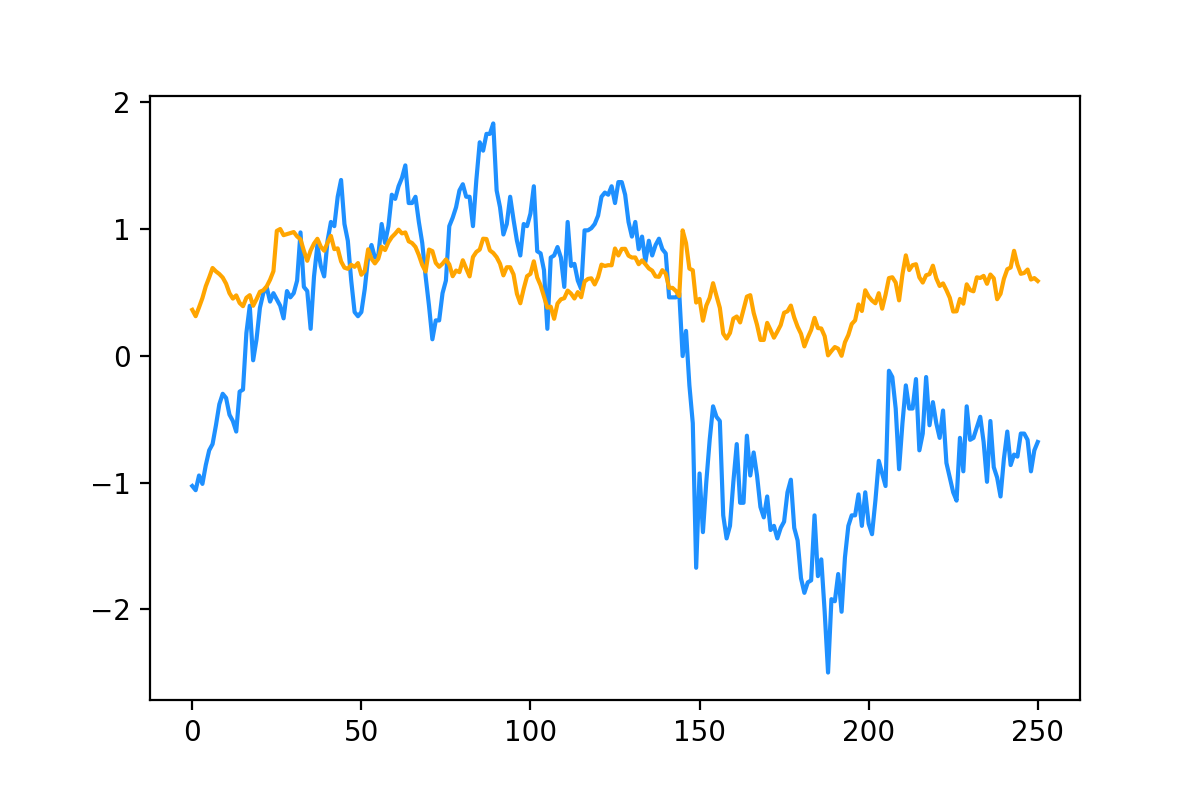
\includegraphics[width=0.3\columnwidth]{zeor2.png} 
    } 
    \caption{ The effect of scaling } 
    \label{fig:scaling1} 
\end{figure} 

